\documentclass[12pt,fleqn]{article}
\usepackage[margin=1in,top=1in,bottom=1in]{geometry}
\usepackage{mathtools}
\usepackage{longtable}
\usepackage{enumitem}
%\usepackage{hyperref}
\usepackage[dvips]{graphics}
\usepackage[table]{xcolor}
\usepackage{amssymb}
\usepackage{float}
\usepackage{booktabs}
\usepackage{tikz}
\usepackage{subcaption}
\usepackage{wrapfig}

\usepackage[normalem]{ulem}

\usepackage{multicol}
\usepackage{txfonts}
%\usepackage{amsfonts}

%%%%%%%%%% bibliography stuff %%%%%%%%%%%%%
%\usepackage[numbers]{natbib}
%\bibliographystyle{abbrvnat}
\usepackage{natbib}
\bibliographystyle{/Users/tonhauser.1/Library/Latex/cslipubs-natbib}

\setlength{\bibhang}{0.5in}
\setlength{\bibsep}{0mm}
\bibpunct[:]{(}{)}{;}{a}{,}{,}
%%%%%%%%%%%%%%%%%%%%%%%%%%%%%%%

\usepackage{wrapfig}

\usepackage{gb4e}
%\usepackage{/Users/judith/Library/Latex/drs}
%\usepackage{/Users/judith/Library/Latex/avm}
\usepackage[all]{xy}
\usepackage{rotating}
\usepackage{tipa}
\usepackage{multirow}
\usepackage{authblk}
\usepackage{adjustbox}
\usepackage{array}

\usepackage{titlesec}
\titleformat*{\section}{\bfseries\footnotesize}
 
\setlength{\parindent}{.3cm}
\setlength{\parskip}{0ex}

\renewcommand\figurename{Fig.}

\newcommand{\yi}{\'{\symbol{16}}}
\newcommand{\nasi}{\~{\symbol{16}}}
\newcommand{\hina}{h\nasi na}
\newcommand{\ina}{\nasi na}

\exewidth{(\thexnumi)}

\newcommand{\citepos}[1]{\citeauthor{#1}'s \citeyear{#1}}
\newcommand{\citetpos}[1]{\citeauthor{#1}'s (\citeyear{#1})}

\newcommand{\6}{\mbox{$[\hspace*{-.6mm}[$}} 
\newcommand{\9}{\mbox{$]\hspace*{-.6mm}]$}}
\newcommand{\sem}[2]{\6#1\9$^{#2}$}
\renewcommand{\ni}{\~{\i}}

\newcommand{\jt}[1]{\textbf{\color{blue}JT: #1}}


\setlength{\belowcaptionskip}{-10pt}


 \begin{document}
  
\begin{center}
{\bf Higher-probability content is more projective than lower-probability content}
\end{center}

\vspace*{-.3cm}

\noindent
A hallmark of the content of the complement (CC) of factive predicates like {\em know}  is that it projects. For example, in an utterance of the sentence \emph{Does Jane know that Sam has a new hat}, the speaker is typically taken to be committed to Sam having a new hat, despite the predicate and the CC being embedded under an entailment-canceling operator (the polar interrogative). The same is typically not true when replacing \emph{know} with a non-factive predicate like \emph{think}. However,  \citealt*{tbd-variability} ({\em Journal of Semantics})  recently showed that there is substantial variability in the projectivity of CCs. While a lot of this variability was explained by the not-at-issueness of the CC, they also found that the lexical content of the CC itself played a role: e.g., the CC \emph{Martha has a new BMW} was less likely to project than \emph{Sam has a new hat}. The authors hypothesized that the projectivity of a CC may depend on its prior subjective probability, such that a CC is more projective the higher its prior probability. The current work finds support for this hypothesis in an experimental investigation of CCs of both factive and non-factive predicates in which the prior probability of the CC was systematically manipulated. We argue that this finding provides support for constraint-based projection analyses that derive the projectivity of utterance content from the integration of multiple cues, including prior CC probability and the meanings of clause-embedding predicates.


\noindent
{\bf Prior probability norming experiment (n = 95):} Prior probability was measured for 20 contents denoted by English sentences (e.g., Julian dances salsa) given a fact that made the content more likely (e.g., Julian is from Cuba) and a fact that made it less likely (e.g., Julian is from Germany). Participants were asked how likely a content is given a fact (e.g., Fact: Julian is from Cuba. How likely is it that Julian dances salsa?) and provided ratings on a sliding scale from `impossible' (interpreted as a probability of 0) to `definitely' (interpreted as a probability of 1). The mean ratings were .7 for high- and .16 for low-probability contents, see Fig.~\ref{f-prior} for the full set of items.

\noindent 
{\bf Projectivity experiment (n=300):} The 20 sentences denoting the normed contents were realized as the complements of 20 clause-embedding predicates, for a total of 400 predicate/complement combinations. These combinations were realized as polar questions with a random subject noun phrase. In the target stimuli, the 400 polar questions were combined with one of the two facts that each content was normed with, for a total of 800 target stimuli. As shown in the sample target stimulus in (\ref{stim}), the named speaker (here, Carol) was explicitly stated to be aware of the fact.
\vspace*{-.6cm}
\begin{wrapfigure}{r}{.31\paperwidth}
\centering
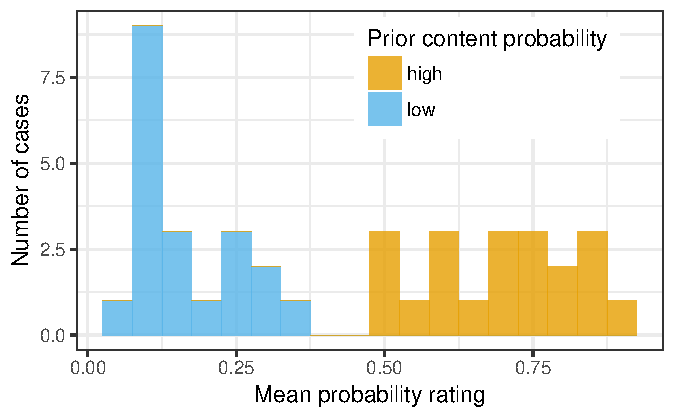
\includegraphics[width=.32\paperwidth]{../results/1-prior/graphs/meanprobratings}
\caption{Histogram of mean prior probability ratings for each item (i.e., content/fact combination). Color indicates whether item was coded as high or low probability in the projectivity analysis.}\label{f-prior}
\end{wrapfigure}%
\begin{exe}
\ex\label{stim}
{\bf Fact (which Carol knows):} Julian is German.  \\ 
{\bf Carol:} Does Sandra know that Julian dances salsa?
\end{exe}
\vspace*{-.15cm}
The 20 predicates included the 5 factives {\em be annoyed, know, see, discover} and {\em reveal}, as well as 15 non-factives: the content of the complement of 9 of these ({\em acknowledge, admit, announce, confess, confirm, establish, hear, inform, prove}) has been described as being able to project (e.g., \citealt{schlenker10,anand-hacquard2014,spector-egre2015,tbd-variability}), in contrast to that of the remaining 6 predicates ({\em pretend, suggest, say, think, be right, demonstrate}).



\noindent Projectivity was measured with the `certain that' diagnostic, following \citealt{tbd-variability}: for (\ref{stim}), participants judged whether Carol is certain that Julian dances salsa. Participants rated 20 target items (one for each predicate) and 6 control items (as attention checks). They responded on a sliding scale from `no' (no projection, coded 0) to `yes' (maximal projection, coded 1).
\begin{wrapfigure}{l}{.45\paperwidth}
\centering
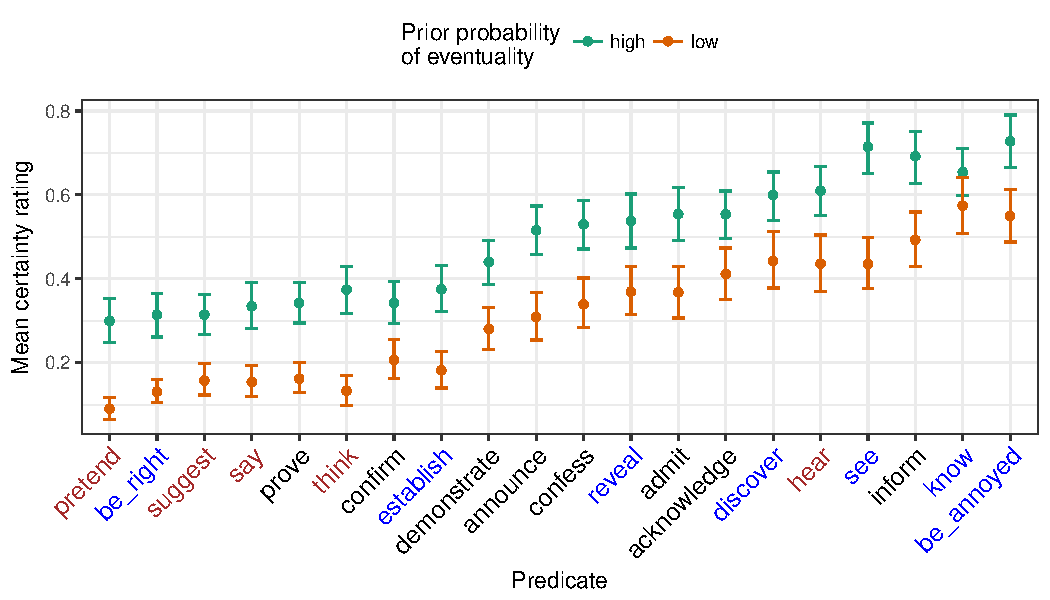
\includegraphics[width=.45\paperwidth]{../results/3-projectivity/graphs/means-projectivity-by-predicate-and-facttype}
\caption{Mean certainty rating by predicate (x-axis) and prior CC probability, with 95\% CIs; factives in green.}\label{f-proj}
\end{wrapfigure}

\noindent
{\bf Results:} Mean certainty ratings for CCs were higher when the content had a higher prior probability (mean: .5) than when the content had a lower prior probability (mean: .32), as predicted by \citetpos{tbd-variability}. As shown in Fig.~\ref{f-proj}, the effect of prior CC probability on projectivity was present across all 20 predicates. We also observe by-predicate variability in certainty ratings:  for instance, the mean certainty ratings for factive {\em be annoyed} were higher, at .72 (high) / .53 (low), than those for factive {\em reveal}, at .55 / .37, which in turn were higher than those for non-factive {\em establish}, at .39 / .19. These findings replicate \citetpos{tbd-variability} finding that projectivity is a gradient property of utterance content.



Linear mixed-effects model predicting certainty rating from fact (high vs.\ low prior probability) and verb, with a random intercept for participant (5520 data points)



\noindent
{\bf Discussion}
\\
Current projection analyses (e.g., \citealt{heim83,vds92,abrusan2011,brst-salt10,brst-ar}) are limited to the projectivity of the content of the complement of factive predicates, to the exclusion of that of non-factive predicates. {\bf But the content of the complement of non-factives may also project, so these analyses don't make predictions about such contents, sad} Our finding for non-factives confirms intuitions by semanticists that but semanticists observed that these contents may nevertheless project (see, e.g., \citealt{schlenker10,anand-hacquard2014,spector-egre2015}). A critical factor in whether the speaker is taken to be committed to such content is the prior probability of the event described by the complement (see, e.g., \citealt{schlenker10}): e.g., the content of the complement of {\em Did Mary announce that she is pregnant} is more likely to project if Mary is a responsible 30-year old than if she is a 7-year old. 

For factive predicates, such analyses can be taken to predict the finding that prior probability influences projectivity. For instance, lexicalist projection analyses (e.g., \citealt{heim83,vds92}) assume default global accommodation when presupposed is not already entailed by or satisfied in the common ground when the trigger is uttered. This default is overridden when the presupposition is inconsistent with information already in the common ground. If we can assume that Julian dancing salsa is more likely to be consistent with the common ground when Julian is from Cuba than when he is from Germany, lexicalist analyses predict that the presupposition that Julian dances salsa is more projective when it has a higher prior probability. Under {\bf non-lexicalist projection analyses}, content is projective when it is by default backgrounded or not-at-issue with respect to the question addressed by the utterance (e.g., \citealt{abrusan2011,abrusan2016,brst-salt10,brst-ar}; \citealt*{tbd-variability}). In a given utterance,  content is more likely to remain backgrounded or to be not-at-issue if it describes a high-probability (i.e., uncontroversial) event than if it describes a low-probability (i.e., controversial) event (e.g., \citealt[252]{simons2003}).

{\bf Implication still needs to be discussed: analysis that integrates multiple cues, not limited to factives}
\newpage

\bibliography{../bibliography}

\end{document}
